\chapter{Prezentacja warstwy użytkowej projektu}

\section{Warstwa Użytkowa Projektu}

Projekt Aplikacji pozwalającej na szybkie sprawdzenie wersji serwisów na serwerach Linux oferuje intuicyjny i prosty w obsłudze interfejs użytkownika, który umożliwia szybkie sprawdzenie wersji serwisów na serwerach Linux.

Aplikacja umożliwia użytkownikom wykonanie następujących akcji:
\begin{itemize}
    \item Sprawdzenie wersji serwisów na danym hoście.
    \item Wywołanie funkcji, która sprawdzi czy wersje serwisów zmieniły się na danym hoście i w razie potrzeby je zaaktualizuje na stronie.
    \item Zmianę wyświetlanych hostów za pomocą przycisków.
\end{itemize}

Interfejs skupia się na minimalizmie i łatwości nawigacji, co pozwala na szybkie odnalezienie potrzebnych informacji i funkcji.

W tej sekcji zostaną umieszczone zrzuty ekranu przedstawiające kluczowe funkcjonalności aplikacji oraz jej interfejs użytkownika.

\begin{figure}[H]
\centering
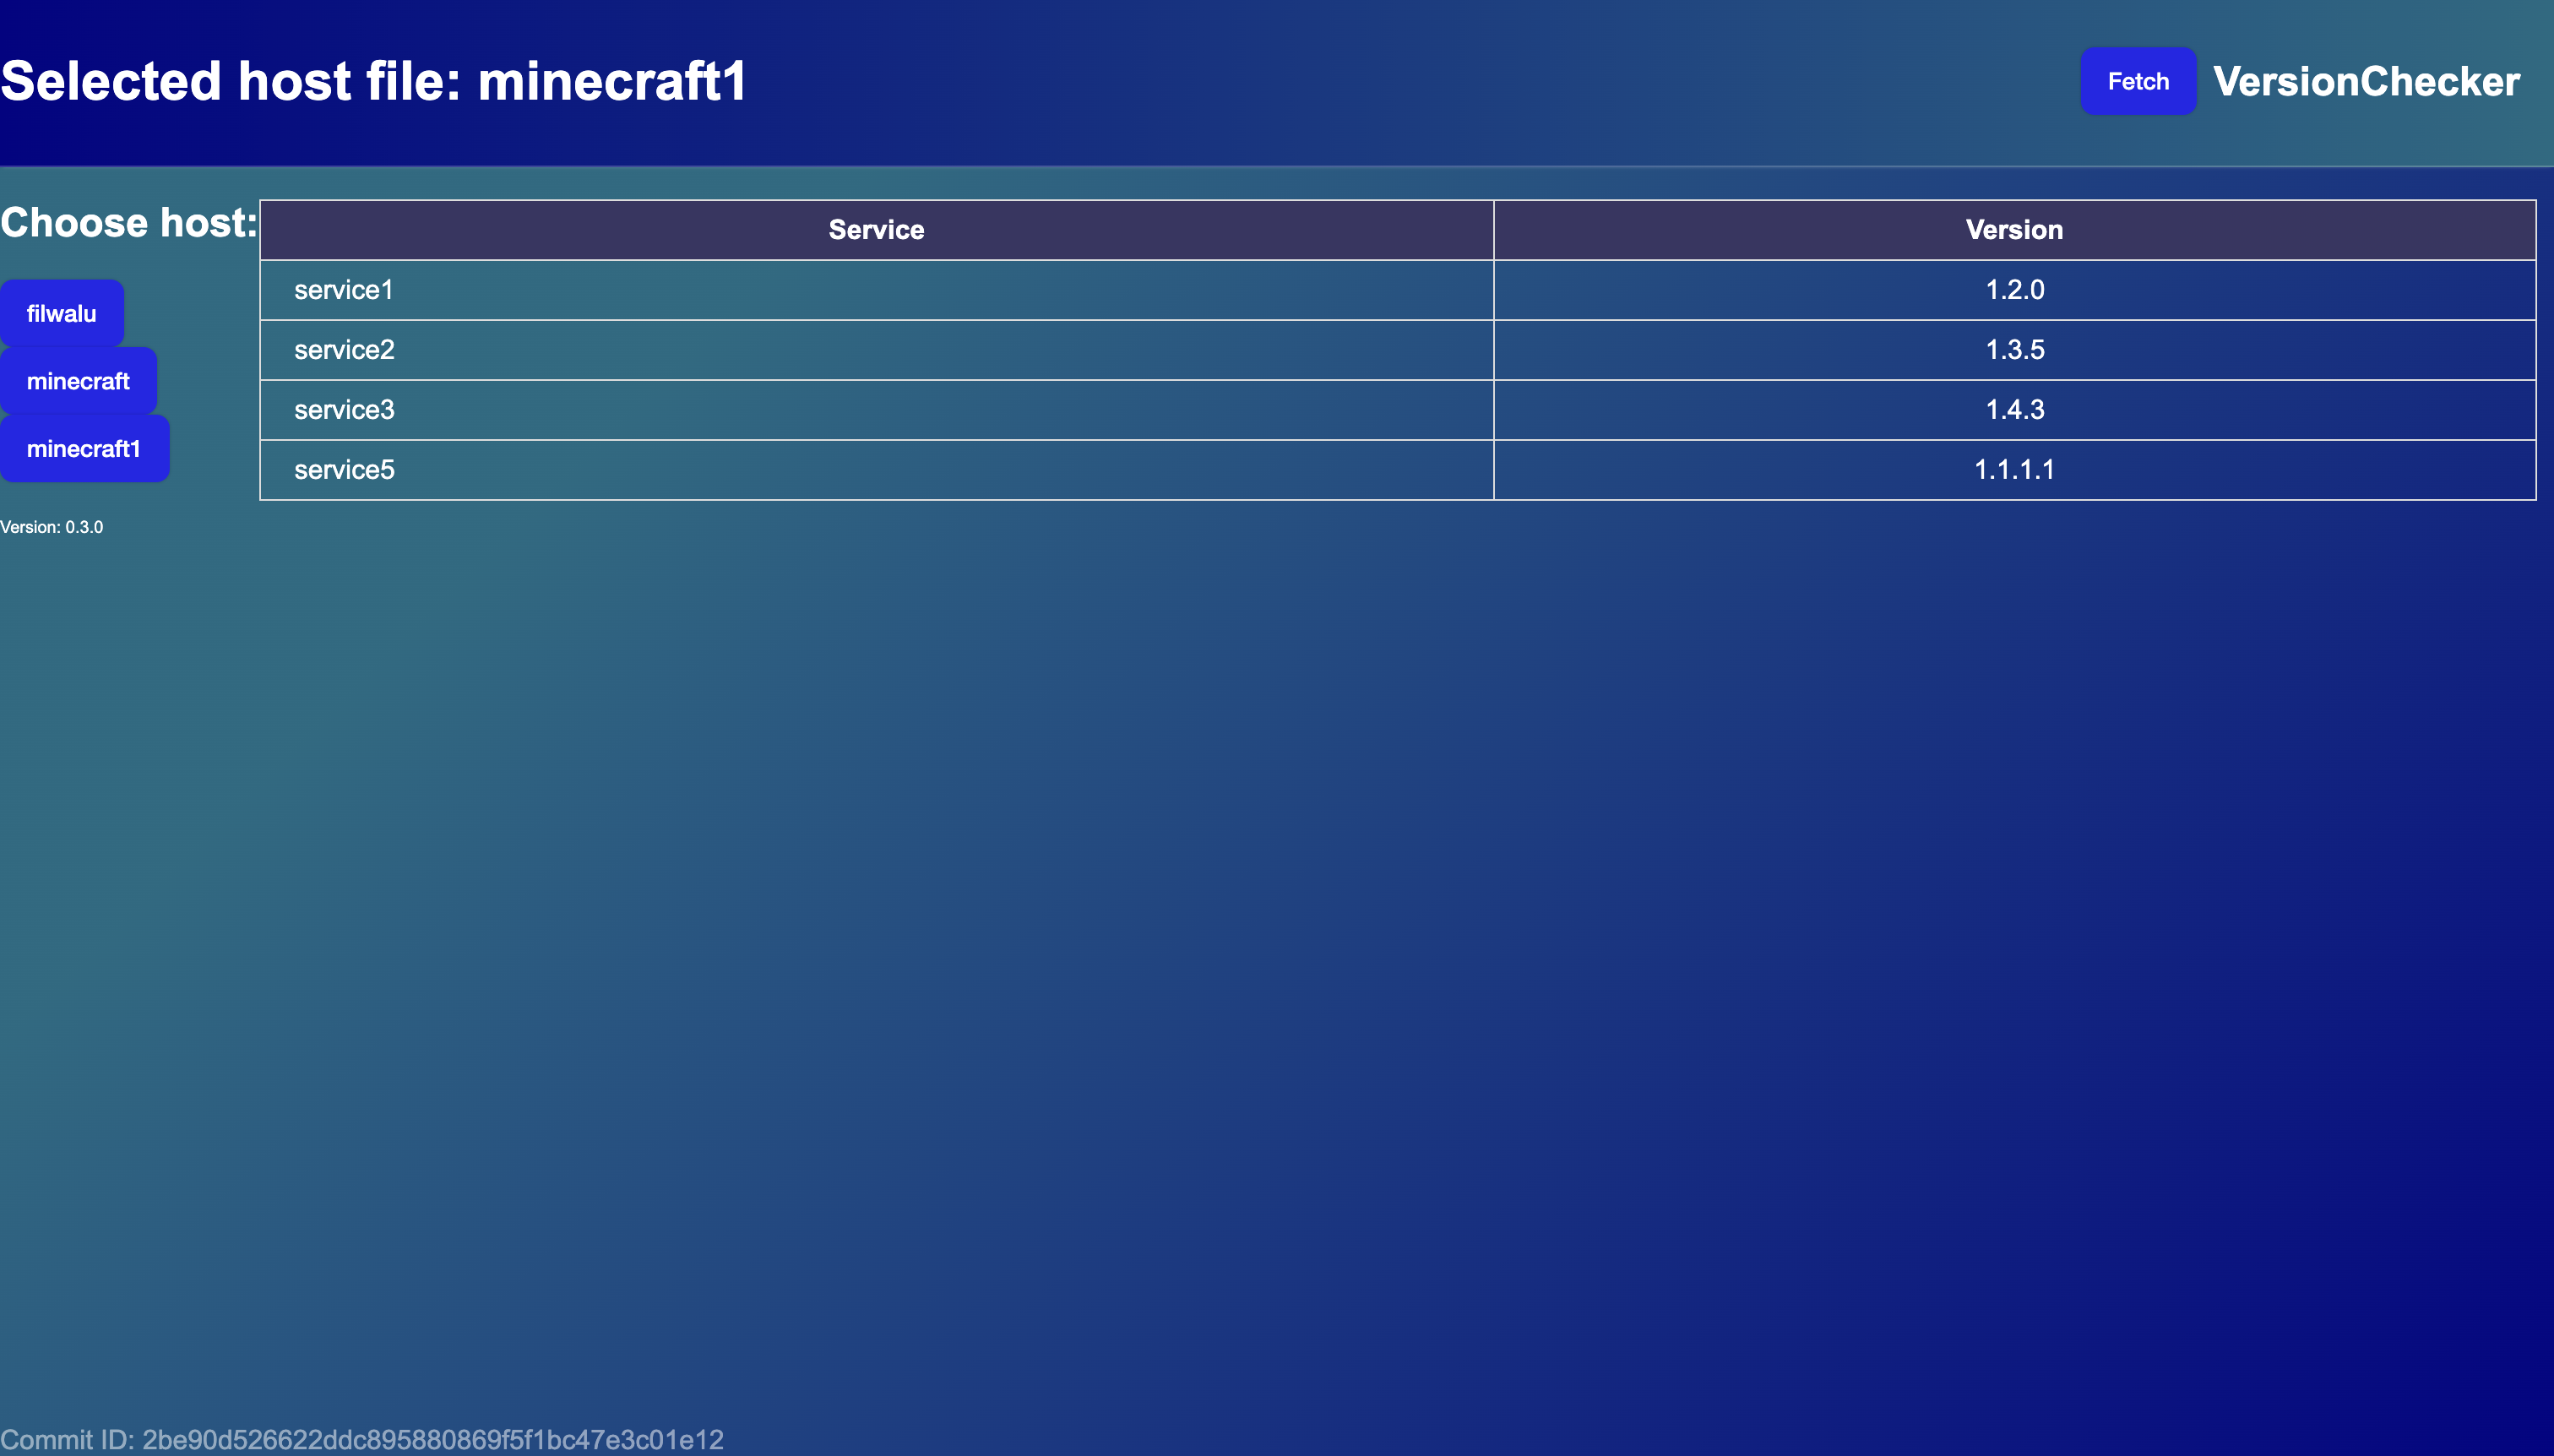
\includegraphics[width=\textwidth]{photos/mainpage.png}
\caption{Strona główna.}
\end{figure}

W tej sekcji omówione zostaną kluczowe funkcjonalności aplikacji instrukcje dotyczące ich używania.

\begin{itemize}
    \item \textbf{Wybór hosta} (\textit{Przyciski z nazwami hostów}):
    Użytkownik może wybrać hosta, którego wersje serwisów chce sprawdzić, klikając na przycisk z nazwą hosta. Po kliknięciu na przycisk, aplikacja wyświetli tabele z nazwami serwisów oraz ich wersjami.
    \begin{figure}[H]
    \centering
    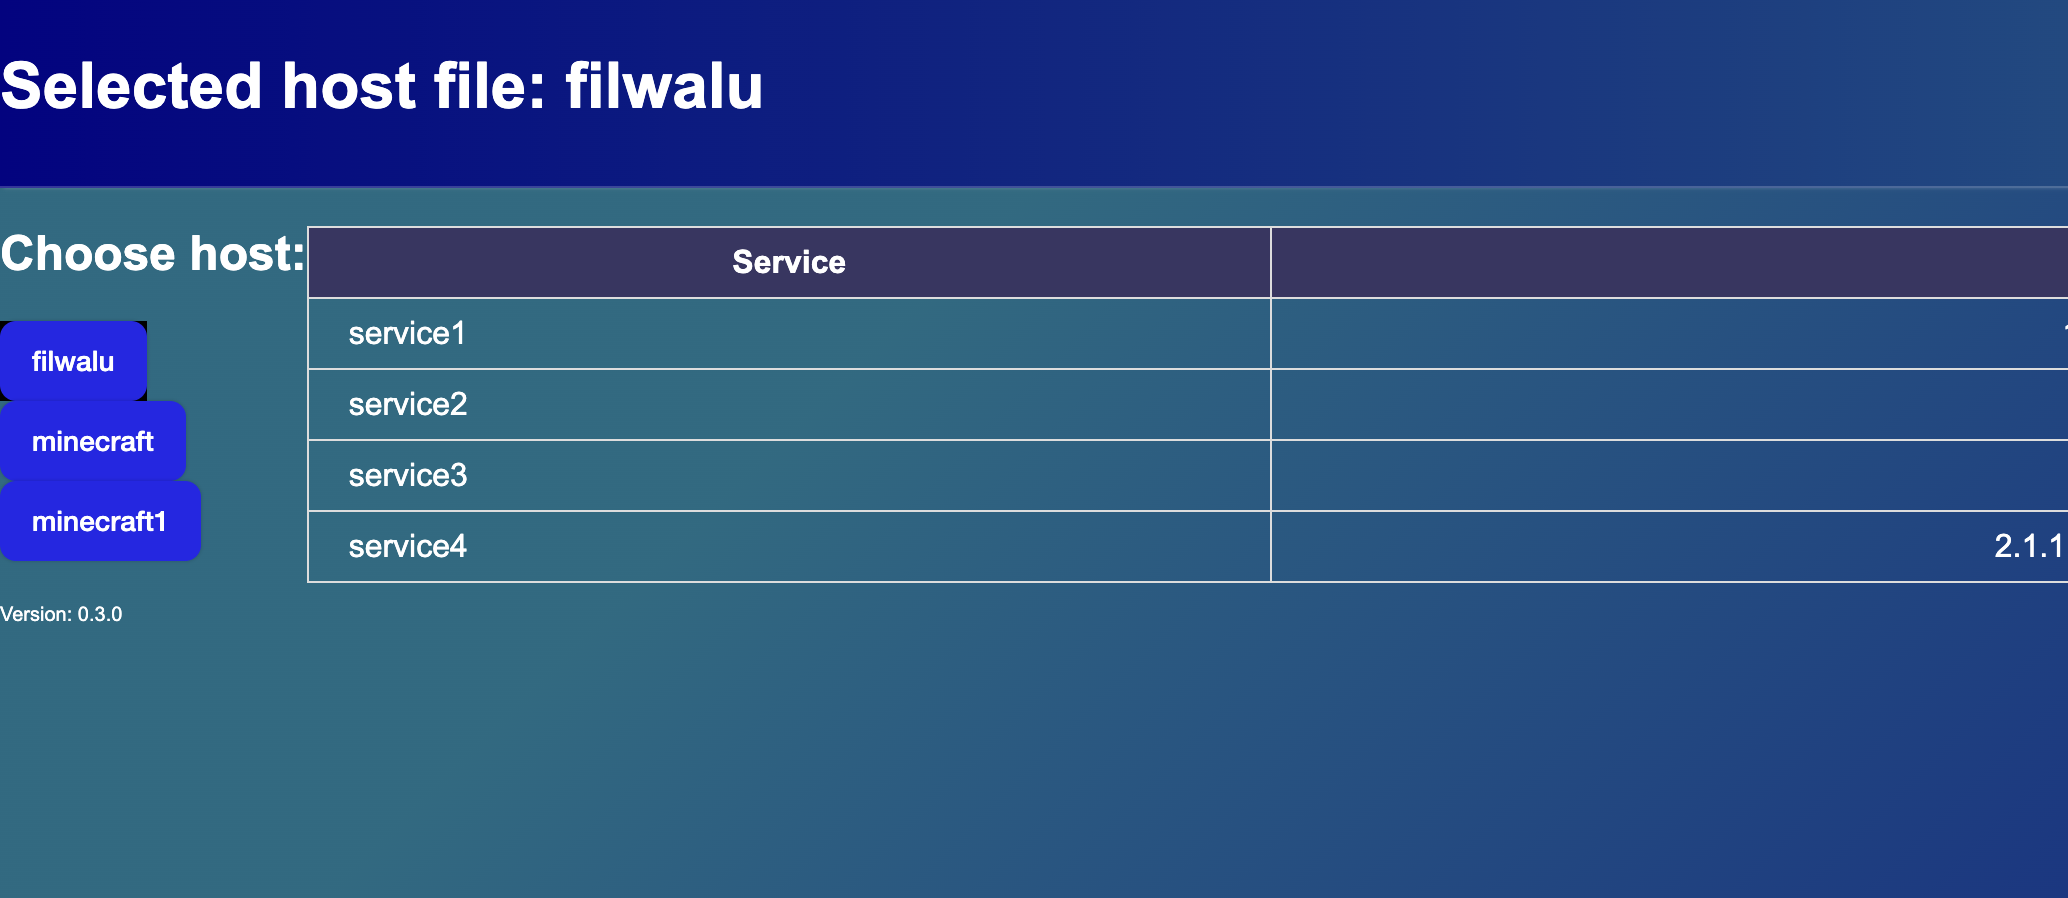
\includegraphics[width=\textwidth]{photos/diffHost.png}
    \caption{Wybór hosta.}
    \end{figure}

    \item \textbf{Pobieranie wersji serwisów} (\textit{Przycisk "Fetch"}):
    Użytkownik może pobrać wersje serwisów dla wybranego hosta, klikając na przycisk "Fetch". Po kliknięciu na przycisk, aplikacja sprawdzi czy wersje serwisów zmieniły się na danym hoście i w razie potrzeby je zaaktualizuje na stronie. 
        \begin{figure}[H]
        \centering
        
\includegraphics[width=\textwidth]{photos/fetchButton.png}
        \caption{Przycisk Fetch.}
        \end{figure}
    \clearpage
    \item \textbf{Status pobierania informacji o wersjach serwisów} (\textit{Komunikat "Update Successful"}):
    Po pobraniu wersji serwisów dla wybranego hosta, aplikacja wyświetli komunikat "Update Successful" informujący użytkownika o pomyślnym pobraniu wersji serwisów.
        \begin{figure}[H]
        \centering
        
\includegraphics[width=\textwidth]{photos/SUCCESS.png}
        \caption{Komunikat Update Successful.}
        \end{figure}

\end{itemize}
\section{Opis interakcji z użytkownikiem}
Aplikacja skupia się na minimalizmie i łatwości nawigacji, co pozwala na szybkie odnalezienie potrzebnych informacji i funkcji. Interfejs użytkownika jest intuicyjny i prosty w obsłudze, dlatego większość błędów jest logowana do pliku app.log. 
